\documentclass[a4paper, 12pt]{article}

\usepackage{wrapfig}
\usepackage{graphicx}
\usepackage{mathtext}
\usepackage{amsmath}
\usepackage{siunitx} % Required for alignment
\usepackage{multirow}
\usepackage{rotating}

\usepackage[T1,T2A]{fontenc}

\usepackage[russian]{babel}
\graphicspath{{pictures/}}


\title{\begin{center}Лабораторная работа №2.2.4\end{center}
Определение коэффицента теплопроводности твердых тел}
\author{Гёлецян А.Г.}
\date{\today}

\begin{document}
    \pagenumbering{gobble}
    \maketitle
    \newpage
    \pagenumbering{arabic}

    \section{Цель работы}
    Определение коэффицентов теплопроводности твердух тел путем сравнения с теплопроводностью эталонного материала, вычисление относительных тепловых потерь через боковые поверхности по измеренным значениям температуры вдоль радиусов пластинок.

    \section{Ход работы}
    \subsection{Теория}
    Количество теплоты, проходящей за еденицу времени через однородную тонкую пластинкой толщиной $\Delta z$ и площадью $S$ при разности температур $\Delta T$ определяется формулой
    \[\Delta q = \kappa S \frac{\Delta T}{\Delta z}\]

    \begin{figure}[h]
        \begin{center}
            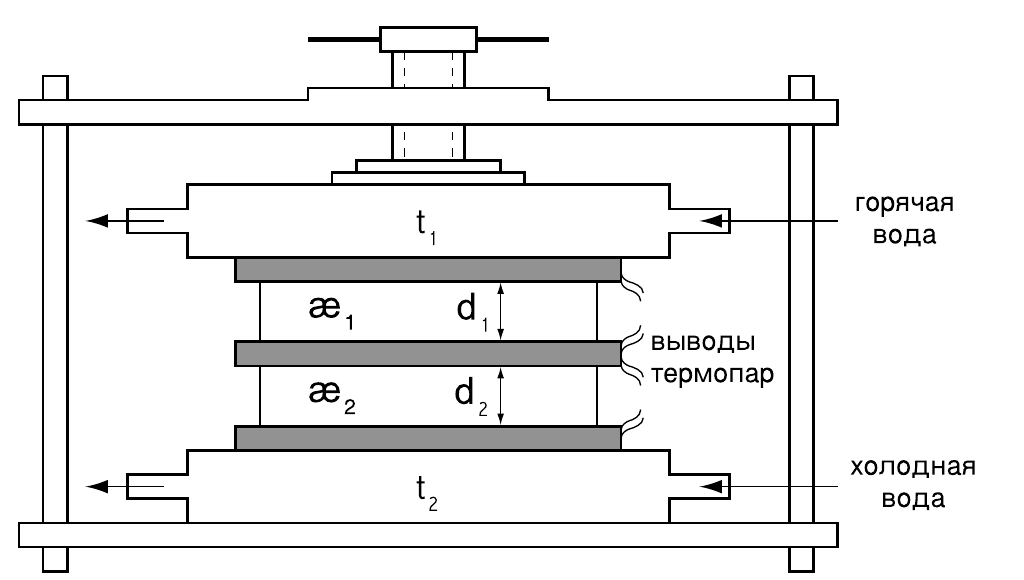
\includegraphics[width=0.8\linewidth]{ustanovka}
            \caption{Схема установки}
        \end{center}
    \end{figure}

    Прямое измерение $\Delta q$ является сложной задачой, поэтому проще сравнить теплопроводность неизвестного материала с эталонным материалом, используя установку на рис. 1. Если пренебречь боковыми потерями, то теплота, проходящая через обе образца будет одинаковой в стационарном режиме. Тогда

    \[\Delta q = \kappa_1 S \frac{\Delta T_1}{\Delta z_1} = \kappa_2 S \frac{\Delta T_2}{\Delta z_2}\]

    откуда получаем

    \begin{equation}
        \frac{\kappa_1}{\kappa_2} = \frac{d_1}{d_2}\frac{\Delta T_2}{\Delta T_1}
    \end{equation}

    Этой формулой и будем пользоваться для сравнения теплопроводностей.

    \subsection{Измерение температур}
    Для измерения температур в работе используются термопары. Напряжение на термопаре
    прямо пропорционально разнице температур между спаем и свободным концом термопары.
    Отсюда вытекает, что
    \[\Delta T \sim \Delta \left(\frac{\varphi}{a}\right)\]
    Где $\varphi$ это напряжение на термопаре, а $a$ это калибровочное напряжение, которое определяется для всех термопар, измеряя напряжение на них при одной и той же разности температур.

    \subsection{Оценка потерь тепла}
    Определим плотность радиального потока тепла $ q_r $. Эта величина определяется радиальным значением градиента температуры. Полный радиальный поток есть произведение $ q_r $ и площади боковой поверхности $ S_r $, вычисленной на том же расстоянии от оси симметрии, на котором производилось измерение радиальной производной температуры

    \begin{equation}\label{poteri1}
    q_r S_r = - \kappa 2 \pi rd \frac{\partial T}{\partial r},
    \end{equation}
    где d -- толщина пластины.

    Полный осевой поток определяется произведением производной температуры вдоль оси симметрии $ z $ и площади окружности, проходящей через точку измерения радиальной производной:

    \begin{equation}\label{poteri2}
    q_z S_z = - \kappa \pi r^2 \frac{\partial T}{\partial z}.
    \end{equation}

    Отношение этих потоков обозначим $ \delta $:

    \begin{equation}\label{poteri3}
    \delta = \frac{2d \frac{\partial T}{\partial r}}{r \frac{\partial T}{\partial z}}.
    \end{equation}

    Этот параметр характеризует расширение теплового потока и его относительные потери, он не зависит от коэффициента теплопроводности.

    Интересно отметить, что величина $ \delta $ не зависит и от радиуса, то есть отношение радиального потока к осевому одинаково и на оси симметрии, и вдали от неё. Расширение осевого теплового потока существует везде, а не только около краев пластинок. Это заключение следует из того, что температура имеет максимум на оси симметрии при любой координате z из-за симметрии пластинок. Поэтому разложение температуры по радиусу от оси начинается с квадратичного члена, следовательно, производная температуры по радиусу в формуле \eqref{poteri3} пропорциональна радиусу, и этот радиус сокращается с радиусом, который уже есть в знаменателе. Кроме того, при малых потерях через боковые стенки осевой поток тепла изменяется тоже на малую величину, поэтому, и производная $ \partial T/\partial z $ изменяется только на малую величину, то есть в первом приближении не зависит от радиуса как и остальные члены формулы \eqref{poteri3}. Отсюда можно сделать вывод, что относительное расширение теплового потока в однородной среде примерно одинаковое на всей пластинке.

    \section{Ход работы}
    \subsection{Измерение относитнльных теплопроводностией}
    \paragraph{}
    В самом начале проговорим, что во всех местах, где был контакт двух различных материалов, между ними ставились резиновые прокладки для увелечения площади соприкосновения образцов. \newline


    Оценим примерное время достижения равновесия, сжав диск гетинакса в установке и измерив зависимость температуры горячей части от времени. Получаем следующее

    \begin{table}[h]
        \begin{center}
            \begin{tabular}{|c|r|r|r|r|r|r|r|r|}
                \hline
                $t, с$ & 0 & 18 & 37 & 70 & 97 & 128 & 180 & 240 \\\hline
                $V, мВ$ & 1.55 & 1.70 & 1.75 & 1.80 & 1.83 & 1.85 & 1.87 & 1.87 \\\hline
            \end{tabular}
        \end{center}
    \end{table}

    Как видим за 4 минуты равновесие было достигнуто. Это и можно принять как характерное время установления равновесия. Т.к. в дальнейшем в установке будут 2 диска, то время ожидания была увеличена до $8\sim10$ мин, исходя из того насколько быстро менялись значения и добавив немного времени для запаса.

    \paragraph{}
    Следующим шагом откалибруем термопары. Для этого зажимаем все термопары между двумя образцами таким образом, чтобы их спаи были максимально близки друг к другу, и по достижению термального равновесия запишем значения вольтметра. Данные приведены в таблице ниже

    \begin{table}[h]
        \begin{center}
            \begin{tabular}{|c|r|r|r|r|}
                \hline
                Номер термопары & 1 &  2 &  3 &  4\\
                \hline
                $a, мВ$ &   0.89 &  0.87 &  0.87 &  0.84\\\hline
            \end{tabular}
        \end{center}
    \end{table}

    После каллибровки начнем основные измерения. Схема измерения уже была описана раньше. Приведем полученные данные.

    \begin{table}[h]
        \begin{center}
            \begin{tabular}{|c|l|rrrr|rrrr|rr|}
                \hline
                {№} & материал & $V1, мВ$ & $V2, мВ$ & $V3, мВ$ & $V4, мВ$ &  №1 &  №2 &  №3 &  №4 &   $d1, мм$ &   $d2, мм$ \\
                \hline
                0 &    eb-eb &  1.10 &  2.07 &  1.10 &  0.11 &   4 &   1 &   3 &   2 &  3.8 &  3.8 \\\hline
                1 &    eb-pg &  1.02 &  2.00 &  1.09 &  0.11 &   4 &   1 &   3 &   2 &  3.8 &  4.8 \\
                2 &    eb-sx &  1.42 &  1.96 &  1.53 &  0.15 &   4 &   1 &   3 &   2 &  3.8 &  1.6 \\
                3 &    eb-tx &  1.22 &  2.04 &  1.28 &  0.13 &   4 &   1 &   3 &   2 &  3.8 &  4.3 \\
                4 &    eb-gx &  1.42 &  2.00 &  1.47 &  0.14 &   4 &   1 &   3 &   2 &  3.8 &  1.8 \\\hline
                5 &    pg-eb &  1.13 &  1.08 &  2.11 &  0.08 &   4 &   1 &   2 &   3 &  4.8 &  3.8 \\
                6 &    sx-eb &  0.70 &  0.64 &  2.06 &  0.14 &   4 &   1 &   2 &   3 &  1.6 &  3.8 \\
                8 &    tx-eb &  0.95 &  0.84 &  2.08 &  0.10 &   4 &   1 &   2 &   3 &  4.3 &  3.8 \\
                7 &    gx-eb &  0.79 &  0.66 &  2.06 &  0.12 &   4 &   1 &   2 &   3 &  1.8 &  3.8 \\
                \hline
            \end{tabular}
        \end{center}
        \caption{Измеренные напряжения на термопарах при различных комбинациях образцов}
    \end{table}

    \paragraph{}
    Немного поясним что за значения в таблице. В столбце "материал" содержится информация об использованных образцах в формате нижний диск - верхний диск. Обазначени: eb - эбонит, pg - плексиглас, sx - стеклотекстолит, tx - текстолит, gx - гетинакс. Слобцы $V1-V4$ показывают напряжение на термопарах, а столбцы $№1-№4$ показывают где была сжата каждая термопара, считая снизу (холодная сторона).
    $d1, d2$ это соответственно толщина нижнего и верхнего диска.

    \paragraph{}
    Используя эти данные по ранее описанны методам считаем отношение теплопроводности исследуемого образца к теплопроводности эбонита.

    \newpage

    \begin{table}[h]
        \begin{center}
            \begin{tabular}{|l|l|ll|ll|l|}
            \hline
            {№} & материал & $\Delta T_1$ & $\Delta T_2$ & $d1, мм$ &   $d2, мм$ & $\kappa / \kappa_{эб}$ \\
            \hline
            0 &    eb-eb &  1.11 &  1.11 &  3.8 &  3.8 &  0.99 \\\hline
            1 &    eb-pg &  1.02 &  1.05 &  3.8 &  4.8 &  1.23 \\
            2 &    eb-sx &  1.42 &  0.49 &  3.8 &  1.6 &  1.21 \\
            3 &    eb-tx &  1.22 &  0.87 &  3.8 &  4.3 &  1.58 \\
            4 &    eb-gx &  1.43 &  0.61 &  3.8 &  1.8 &  1.11 \\\hline
            5 &    pg-eb &  1.17 &  1.18 &  4.8 &  3.8 &  1.27 \\
            6 &    sx-eb &  0.62 &  1.63 &  1.6 &  3.8 &  1.11 \\
            8 &    tx-eb &  0.95 &  1.43 &  4.3 &  3.8 &  1.70 \\
            7 &    gx-eb &  0.74 &  1.61 &  1.8 &  3.8 &  1.02 \\
            \hline
            \end{tabular}
            \caption{Отношение теплопроводностей образцов к теплопроводности эбонита}
        \end{center}
    \end{table}

    Разности температур считаем по формуле

    \[T_1 = \frac{V_2}{a_2} - \frac{V_1}{a_1}\]
    \[T_2 = \frac{V_2}{a_4} - \frac{V_1}{a_3}\]

    \paragraph{}
    Как видим в номере 0 у эбонита теплопроводность не меняется в данном диапазоне температур. Однако строго судить об остальных величинах без подсчета погрешностей и учета утечки теплоты с боковых граней.

    \paragraph{}
    С начала посчитаем погрешность вычислении. Все вычисления по стандартным формулам. Посчитав получаем

    \begin{table}[h]
        \begin{center}
        \begin{tabular}{|l|l|ll|}
        \hline
        {№} & материал &    $\kappa / \kappa_{эб}$ & $\Delta(\kappa / \kappa_{эб})$ \\
        \hline
        0 &    eb-eb &  0.99 &  0.05 \\\hline
        1 &    eb-pg &  1.23 &  0.03 \\
        2 &    eb-sx &  1.21 &  0.06 \\
        3 &    eb-tx &  1.58 &  0.01 \\
        4 &    eb-gx &  1.11 &  0.06 \\\hline
        5 &    pg-eb &  1.27 &  0.06 \\
        6 &    sx-eb &  1.11 &  0.09 \\
        8 &    tx-eb &  1.70 &  0.08 \\
        7 &    gx-eb &  1.02 &  0.07 \\
        \hline
        \end{tabular}

        \end{center}
        \caption{относительные теплопроводности и их ошибки}
    \end{table}

    \paragraph{}
    Как видим ошибки (систематические) довольно большие, и для одно и того же материала теплопроводности при разных температурах имеют перекрытие погрешностей, поэтому наш опыт не имеет достаточной точности чтобы определить зависимость теплопроводности от температуры. Единственные значения где нет перекрытия это значения текстолита, но и это тоже спорно.

    \subsection{Оценка боковых потерь}

    Прижмем в установке диски текстолита (снизу) и эбонита (сверху).Прикрепим к верхней (горячей) стороне текстолитового диска термопары так, как показано на рисунке. Измерим значения наряжений на термопарах. Построим график зависимости относительной температуры от расстояния до центра диска.

    \begin{figure}[h]
        \begin{center}
            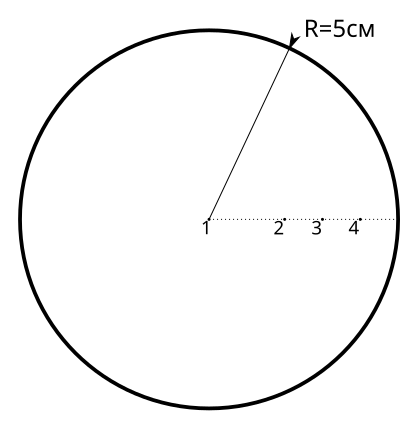
\includegraphics[width=0.5\linewidth]{radial}
        \end{center}
    \end{figure}

    Получаем следующую картину.

    \begin{table}[h]
        \begin{center}
            \begin{tabular}{|c|r|r|r|r|}
                \hline
                Номер термопары & 1 &  2 &  3 &  4\\
                \hline
                $V, мВ$ &   0.87 &  0.83 &  0.86 &  0.76\\
                \hline
                $T$ & 0.9775 & 0.9540 & 0.9885 & 0.9048\\
                \hline
            \end{tabular}
            \caption{Засисимоть температуры от расстояния до центра}
        \end{center}
    \end{table}

    Как видим третья чувтвует себя не очень, поэтому будет разумно убрать его. Считая что зависимость квадратичная, примерно можем написать

    \begin{equation}
        \frac{\partial T}{\partial r}(r=4см) \approx \frac{2(T_4-T_1)}{4см} = -0.036 см^{-1}
    \end{equation}

    \begin{figure}[h]
        \begin{center}
            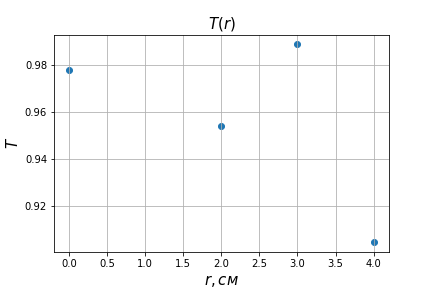
\includegraphics[width=\linewidth]{T_r}
        \end{center}
        \caption{График радиальной зависимости температуры $(T=V/a)$}
    \end{figure}

    Для текстолита, из прошлых данных имеем что
    \begin{equation}
        \frac{\partial T}{\partial z} \approx \frac{\Delta T}{d} = \frac{0.95}{4.3мм} = 2.21 см^{-1}
    \end{equation}
    Подставляя все это в формулу (\ref{poteri3}) получаем
    \begin{equation}\label{poteri4}
        \delta = \frac{2d |\frac{\partial T}{\partial r}|}{r \frac{\partial T}{\partial z}} \approx 0.3\%
    \end{equation}
    Как видим эта поправка несколько раз меньше относительной систематической ошибки, поэтому ею можем пренебречь и записать полную ошибку как систематическую.

    \section{Заключение}
    \paragraph{}
    Как видим основной проблемой данной установки является низкая точность измерения температуры, из за чего относительные теплопроводности имеют большие погрешности. В рамках опыта зависимости теплопроводности от температуры не выявлена. Боковые потери пренебрежимо малы в сравнении с другими неточностями установки.
\end{document}



